% Copyright 2004 by Till Tantau <tantau@users.sourceforge.net>.
%
% In principle, this file can be redistributed and/or modified under
% the terms of the GNU Public License, version 2.
%
% However, this file is supposed to be a template to be modified
% for your own needs. For this reason, if you use this file as a
% template and not specifically distribute it as part of a another
% package/program, I grant the extra permission to freely copy and
% modify this file as you see fit and even to delete this copyright
% notice. 

\documentclass{beamer}

\usepackage{blindtext}
\usepackage{tcolorbox}
\usepackage{soul}

\usepackage{amsmath}
\usepackage{amssymb}
\usepackage{amsthm}
\usepackage{amsfonts}

\makeatletter
\newcommand\xleftrightarrow[2][]{%
  \ext@arrow 9999{\longleftrightarrowfill@}{#1}{#2}}
\newcommand\longleftrightarrowfill@{%
  \arrowfill@\leftarrow\relbar\rightarrow}
\makeatother

\usefonttheme{professionalfonts} % using non standard fonts for beamer
\usefonttheme{serif} % default family is serif
%\usepackage{fontspec}
%\setmainfont{Liberation Serif}

% There are many different themes available for Beamer. A comprehensive
% list with examples is given here:
% http://deic.uab.es/~iblanes/beamer_gallery/index_by_theme.html
% You can uncomment the themes below if you would like to use a different
% one:
%\usetheme{AnnArbor}
%\usetheme{Antibes}
%\usetheme{Bergen}
%\usetheme{Berkeley}
%\usetheme{Berlin}
%\usetheme{Boadilla}
%\usetheme{boxes}
%\usetheme{CambridgeUS}
%\usetheme{Copenhagen}
%\usetheme{Darmstadt}
\usetheme{default}
%\usetheme{Frankfurt}
%\usetheme{Goettingen}
%\usetheme{Hannover}
%\usetheme{Ilmenau}
%\usetheme{JuanLesPins}
%\usetheme{Luebeck}
%\usetheme{Madrid}
%\usetheme{Malmoe}
%\usetheme{Marburg}
%\usetheme{Montpellier}
%\usetheme{PaloAlto}
%\usetheme{Pittsburgh}
%\usetheme{Rochester}
%\usetheme{Singapore}
%\usetheme{Szeged}
%\usetheme{Warsaw}



\title{Introduction to Signal Processing}

% A subtitle is optional and this may be deleted
\subtitle{Lecture 5: \textbf{Laplace Transform and its Properties}}

\author{Sivakumar Balasubramanian}
% - Give the names in the same order as the appear in the paper.
% - Use the \inst{?} command only if the authors have different
%   affiliation.

\institute[Christian Medical College] % (optional, but mostly needed)
{
  \inst{}%
  Department of Bioengineering\\
  Christian Medical College, Bagayam\\
  Vellore 632002
}
% - Use the \inst command only if there are several affiliations.
% - Keep it simple, no one is interested in your street address.

\date{}
% - Either use conference name or its abbreviation.
% - Not really informative to the audience, more for people (including
%   yourself) who are reading the slides online

\subject{Lecture notes on signal processing}
% This is only inserted into the PDF information catalog. Can be left
% out.

% If you have a file called "university-logo-filename.xxx", where xxx
% is a graphic format that can be processed by latex or pdflatex,
% resp., then you can add a logo as follows:

% \pgfdeclareimage[height=0.5cm]{university-logo}{university-logo-filename}
% \logo{\pgfuseimage{university-logo}}

% Delete this, if you do not want the table of contents to pop up at
% the beginning of each subsection:
\AtBeginSubsection[]
{
  \begin{frame}<beamer>{Outline}
    \tableofcontents[currentsection,currentsubsection]
  \end{frame}
}

% Let's get started
\begin{document}

\begin{frame}
  \titlepage
\end{frame}

% READING MATERIAL
\begin{frame}{Reading material}

\begin{itemize}
\item Chapter 6 from reference [2]
\item Chapter 9 from reference [3]
\end{itemize}

\end{frame}


% LAPLACE TRANSFORM
\begin{frame}{Laplace transform}

\begin{itemize}
\item For an LTI system, we saw that the following is true,
\[ y(t) = e^{st}\left(\int_{-\infty}^{\infty}h(\tau)e^{-s\tau}d\tau\right) \]
\item This naturally led to the Fourier transform, where $s = j\omega$.
\item There is no restriction on $s$ to be purely imaginary. One would obtain a more general transform by assuming, $s=\sigma  + j\omega \,\,\, \longrightarrow$ \textit{Laplace transform}.
\item The Fourier transform which was a tool to decompose a given signal $x(t)$ into different complex exponentials $e^{j\omega}$. 
\item What does the Laplace transform do? i.e. when $s=\sigma + j\omega$?
\end{itemize}
\end{frame}

% LAPLACE TRANSFORM
\begin{frame}{Laplace transform}

\begin{itemize}
\item Laplace transform decomposes a given signal $x(t)$ into exponential growing or decaying sinusoids.
\[ X(s) = \mathcal{L}\left\lbrace x(t) \right\rbrace \triangleq \int_{-\infty}^{\infty}x(t)e^{-st}dt; \,\,\, x(t) \xleftrightarrow{\mathcal{L}} X(s) \]

\vspace{-5mm}
\begin{figure}
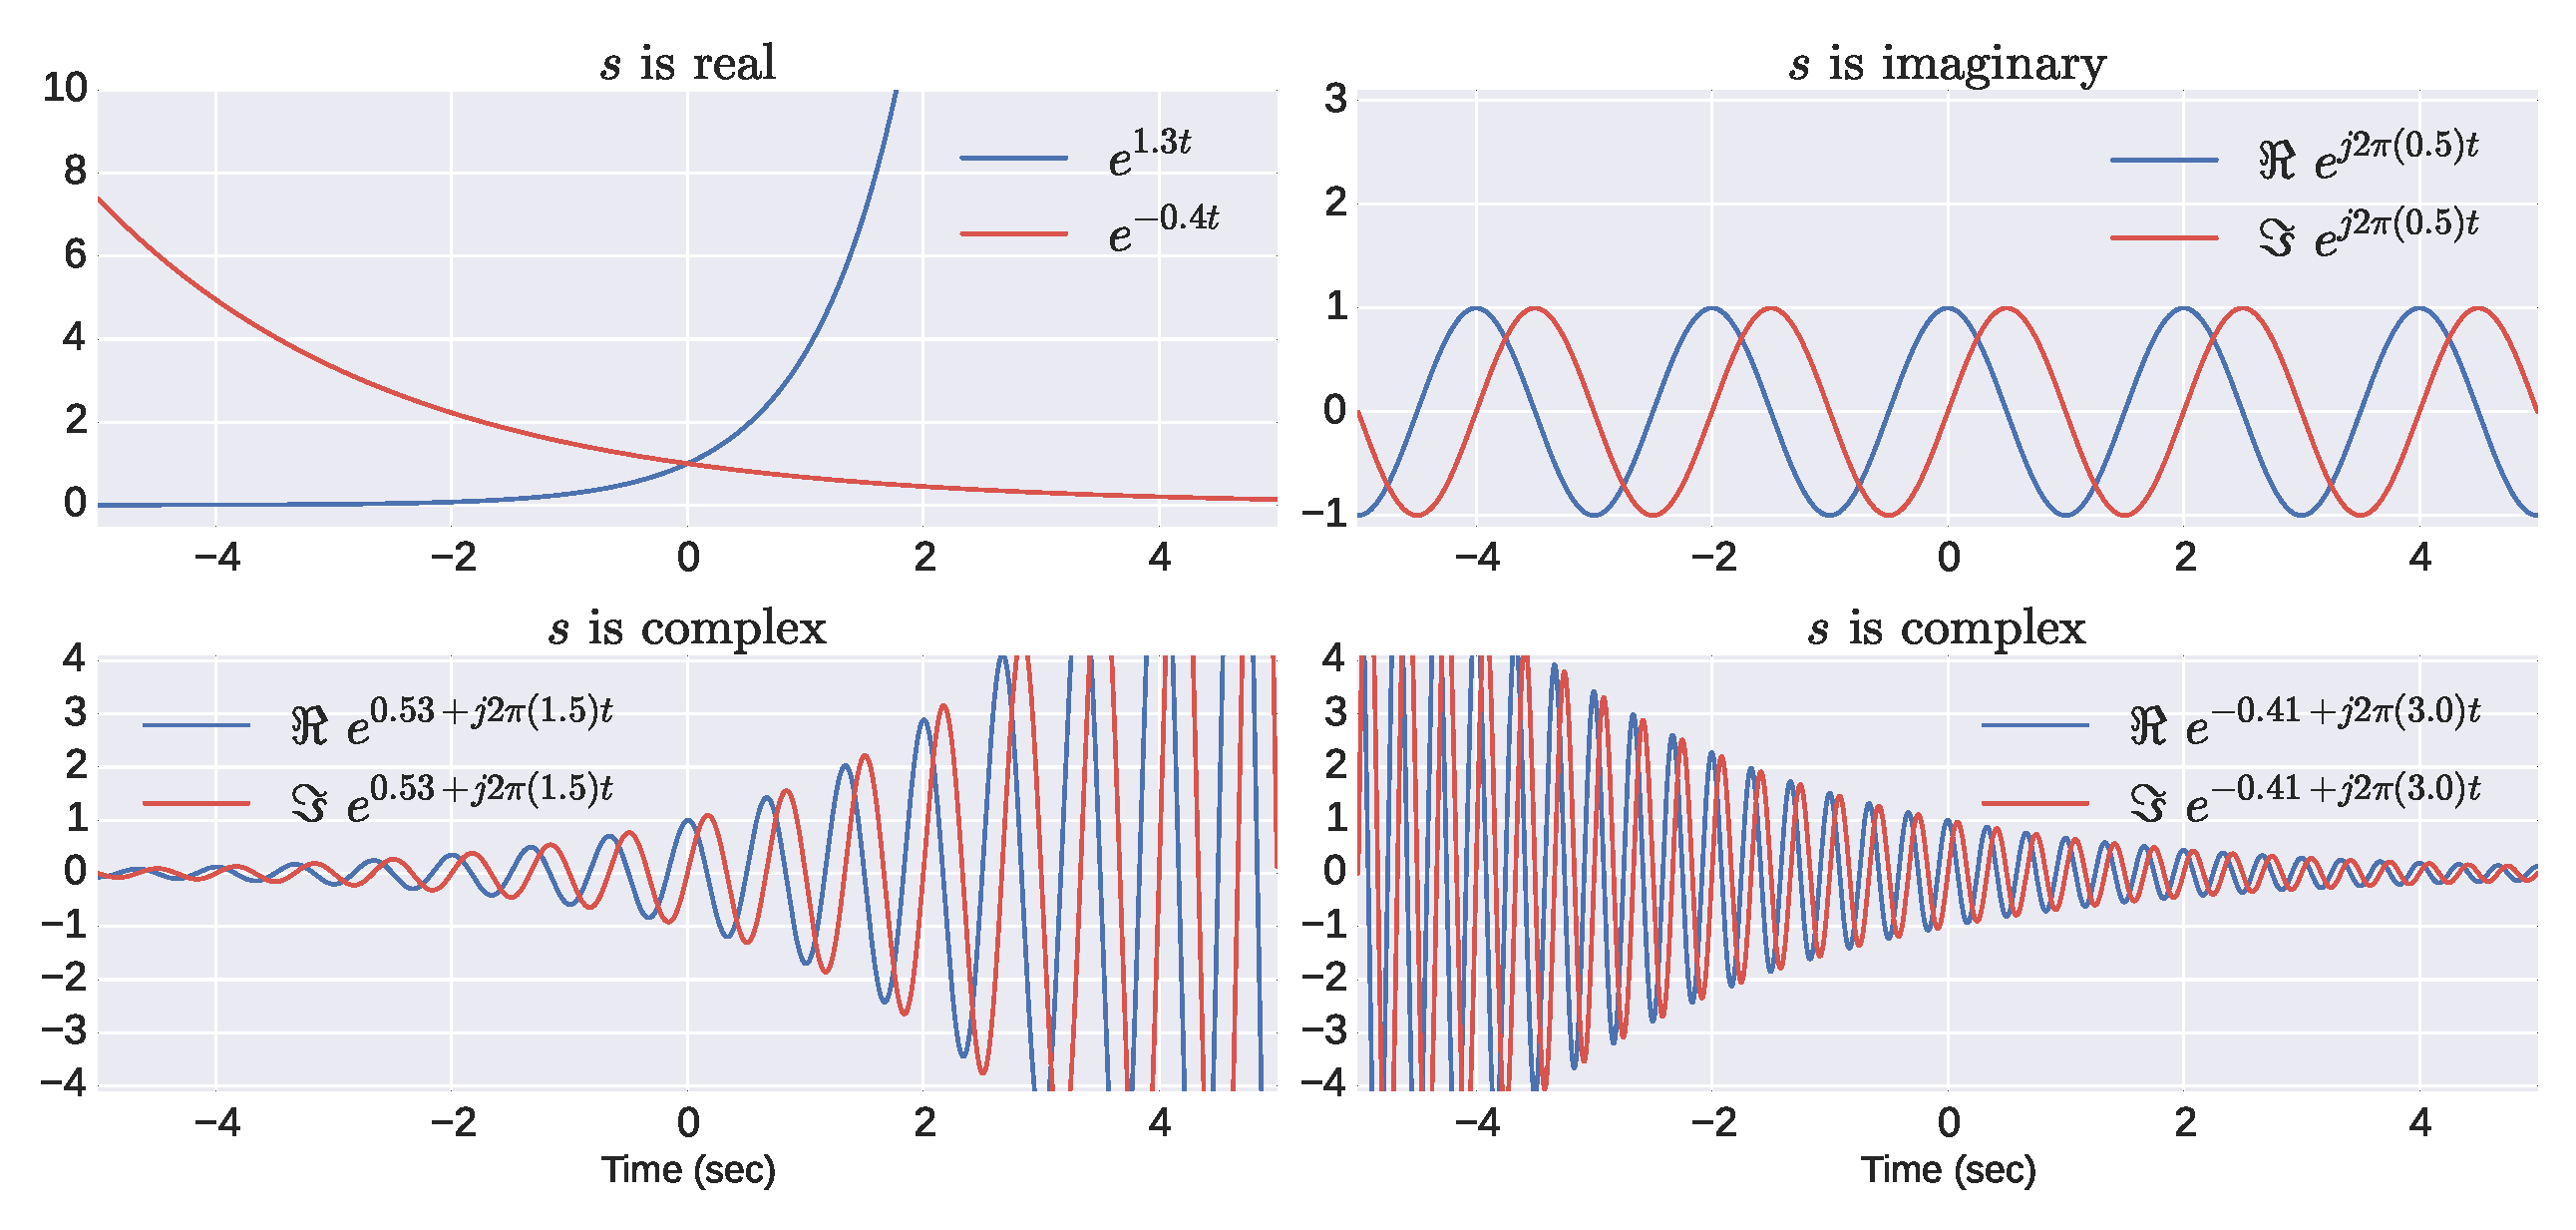
\includegraphics[width=0.9\textwidth]{img/complex_exp.eps}
\end{figure}

\item Fourier transform can be obtained from Laplace transform, $X(s)\Big|_{s=j\omega}$.
\end{itemize}
\end{frame}

% LAPLACE TRANSFORM
\begin{frame}{Laplace transform}

\begin{itemize}
\item Another way to look at the Laplace transform is the following,
\[ X(\sigma + j\omega) = \int_{-\infty}^{\infty}\left(x(t)e^{-\sigma t}\right) e^{-j\omega t}dt \]
\item Laplace transform can be see as the Fourier transform of $x(t)e^{-\sigma t}$. 
$$x(t) \xleftrightarrow{\mathcal{L}} X(s) \xleftrightarrow{\mathcal{F}} x(t)e^{-\sigma t}$$ 
\item Just like the Fourier transform, the Laplace transform exists if the above integral converges. The convergence of this integral can be controlled by the factor $\sigma$.
\item To understand this, evaluate the Laplace transform of $x(t) = e^{\alpha t}u(t)$. Does the Laplace transform exist for all values of $s$?
\end{itemize}
\end{frame}

% LAPLACE TRANSFORM
\begin{frame}{Laplace transform}

\begin{itemize}
\item The set of all $s$ (with the corresponding $\sigma$) for which the Laplace transform exists, is the called the \textit{Region of convergence (ROC)}.
\item A complete specification of a signal's Laplace transform requires the specification of $X(s)$ and the ROC.
\item Why is this? You can understand this by evaluating the Laplace transforms of the following:
\[ x_1(t) = e^{at}u(t) \,\,\, \text{and} \,\,\, x_2(t) = -e^{-at}u(-t) \]

What are their Laplace transforms and their ROCs? This should make it clear why the ROC is essential.
\end{itemize}
\end{frame}

% UNILATERAL LAPLACE TRANSFORM
\begin{frame}{Unilateral Laplace Transform}

\begin{itemize}
\item Laplace transform is often used as a tool to analyse LTI systems, through the Laplace transform of their impulse response.
\[ H(s) = \mathcal{L}\left\lbrace h(t) \right\rbrace = \int_{-\infty}^{\infty} h(t) e^{-st}dt \]

$H(s)$ is called the transfer function of the LTI system.

\item We are often only interested in systems that are causal, i.e. impulse responses that are one-sided. $h(t) = 0, \forall t < 0$. For such cases, we define a modified version of the Laplace transform, called the \textit{unilateral} Laplace transform,
\[ H(s) = \mathcal{L}_{-}\left\lbrace h(t) \right\rbrace \triangleq \int_{0^{-}}^{\infty} h(t) e^{-st}dt \]

The lower limit is set to $0^{-}$ because this enables the transform to take into the initial conditions in a system. This will be made more clear later.

\end{itemize}

\end{frame}

% TRANSFER FUNCTION
\begin{frame}{Transfer Function}

Evaluate the Laplace transforms of the following impulse responses:
\begin{itemize}
\item $h(t) = e^{-t/\tau} u(t), \,\, \tau > 0$
\item $h(t) = a_1e^{-t/\tau_1}u(t) + a_2e^{-t/\tau_2}u(t), \,\, \tau_1 > 0 \, \text{and} \, \tau_2 > 0$
\item $h(t) = e^{-\alpha t}\sin 2\pi\omega t, \,\, \alpha > 0$
\item $h(t) = e^{\beta t}, \,\, \beta > 0 $
\end{itemize}

A common feature you will find from the Laplace transforms of all these impulse responses is that they are all rational polynomials of the following form,
\[ H(s) = \frac{B(s)}{A(s)} \]

The roots of the two polynomial $B(s)$ and $A(s)$ are called the \textit{zeros} and \textit{poles} of the transfer function.
\end{frame}

% TRANSFER FUNCTION
\begin{frame}{Transfer Function}

\[ H(s) = \frac{B(s)}{A(s)} = \frac{b_Ms^M + b_{M-1}s^{M-1} + \cdots b_0}{a_Ns^N + a_{N-1}s^{N-1} + \cdots a_0}\]

\[ H(s) = K\frac{\left(s - z_1\right)\left(s - z_2\right)\cdots\left(s - z_M\right)}{\left(s - p_1\right)\left(s - p_2\right)\cdots\left(s - p_N\right)}; \,\,\, K=\frac{b_M}{a_N}\]

Where the $z_i$s and $p_i$s are the zeros and poles of the transfer function, respectively.
\vspace{5mm}

\textbf{Zeros}: $\lim_{s \to z_i} H(s) = 0$ and \textbf{Poles}: $\lim_{s \to p_i} H(s) = \infty$
\vspace{5mm}

The poles and zeros of a transfer function can visualized on the complex $s$ plane with $\sigma$ as the abscissa and $\omega$ as the ordinate.
\vspace{5mm}

$z_i$ is presented as a '$\text{o}$' and $p_i$ is represented as a '$\times$'.
\end{frame}

% S PLANE
\begin{frame}{$s$ plane}

Consider the following transfer function.
\[ H(s) = \frac{(s-1)(s+2)}{(s-\frac{3}{4})(s^2 + s + 1)} = \frac{(s-5)(s+2)}{(s-\frac{3}{4})(s +\frac{1}{2} - j\frac{\sqrt{3}}{2})(s +\frac{1}{2} + j\frac{\sqrt{3}}{2})}\]

\vspace{-5mm}
\begin{figure}
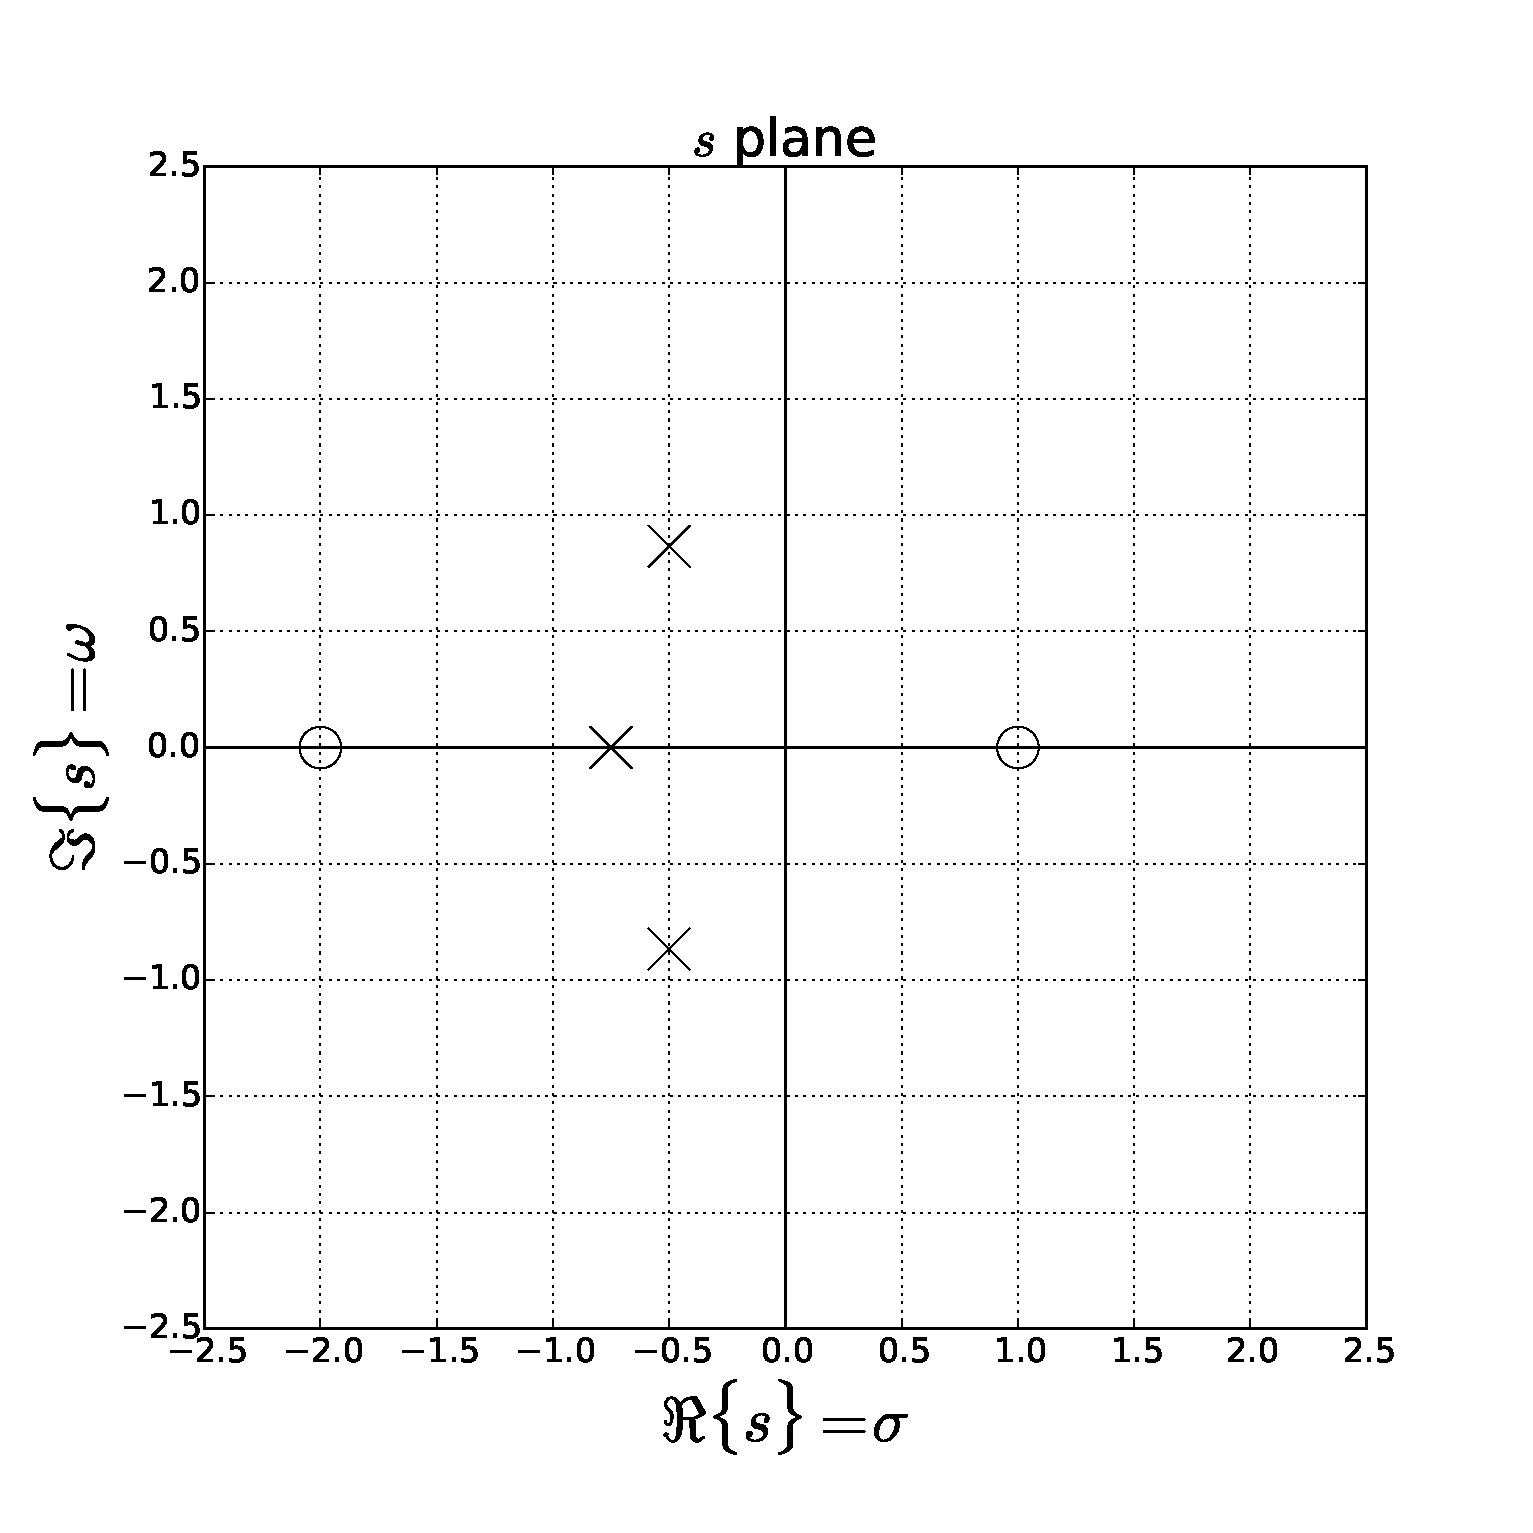
\includegraphics[width=0.6\textwidth]{img/splane.eps}
\end{figure}

\end{frame}

% PROPERTIES OF THE ROC
\begin{frame}{Properties of the ROC}

\begin{small}
\begin{itemize}
\item The ROC is always a strip parallel to the imaginary axis ($j\omega$ axis).\\
\textit{This this because the convergence properties of the Laplace transform for a signal are determined only by $\Re \left\lbrace s \right\rbrace = \sigma$.}
\item For rational Laplace transforms, the ROC does not contain any poles.\\
\textit{If the ROC has any poles, then it would contain a point where the Laplace transform integral does not converge.}
\item For a right sided signal\footnote{The value of the signal is zero prior to a finite time value $T$.}, if a point $\Re \left\lbrace s \right\rbrace = \sigma$ is in the ROC, then all points $\Re \left\lbrace s \right\rbrace > \sigma$ are also in the ROC.
\item For a left sided signal\footnote{The value of the signal is zero after to a finite time value $T$.}, if a point $\Re \left\lbrace s \right\rbrace = \sigma$ is in the ROC, then all points $\Re \left\lbrace s \right\rbrace < \sigma$ are also in the ROC.
\item If the signal is two sided\footnote{Extends to infinitely along both positive and negative time.}, then the ROC is restricted to a strip, such that $\sigma_1 < \Re \left\lbrace s \right\rbrace < \sigma_2$.
\item For a finite duration signal, if there is at least one value of $s$ in the ROC, then the entire $s$-plane is in the ROC.
\end{itemize}
\end{small}
\end{frame}

% INVERSE LAPLACE TRANSFORM
\begin{frame}{Inverse Laplace Transform}

How does one would recover the time domain signal from a Laplace transform? $X(s)$ is the Fourier transform of $x(t)e^{-\sigma t}$ for some fixed $\sigma = \Re \left\lbrace s \right\rbrace, s \in \text{ROC}$. 

So, the inverse Laplace transform can be obtained by taking the inverse Fourier transform of $X(\sigma + j\omega)$.
\vspace{-2mm}
\[ x(t)e^{-\sigma t} = \frac{1}{2\pi} \int_{-\infty}^{\infty}X(\sigma + j\omega)e^{j\omega t} d\omega \]
\vspace{-2mm}
\[ x(t) = \frac{1}{2\pi} \int_{-\infty}^{\infty}X(\sigma + j\omega)e^{\sigma + j\omega t} d\omega \]

Let $\sigma + j\omega = s \, \implies \, jd\omega = ds$. Then the \textit{inverse Laplace transform} is given by,
\vspace{-4mm}
\[ x(t) = \frac{1}{2\pi j} \int_{\sigma - j\infty}^{\sigma + j\infty}X(s)e^{st}ds \]

For most practical purposes, the above complex integral need not be computed. We simply make use of table of standard transform pairs and properties of Laplace transform to obtain the inverse. 
\end{frame}

% PROPERTIES OF LAPLACE TRANSFORM
\begin{frame}{Properties of Laplace transform}

\begin{itemize}
\item \textbf{Linearity:} Let, $x_1(t) \xleftrightarrow{\mathcal{L}} X_1(s), \, s \in R_1$ and $x_2(t) \xleftrightarrow{\mathcal{L}} X_2(s), \, s \in R_2$. Then,
\vspace{-3mm}
\[ a_1x_1(t) + a_2x_2(t) \xleftrightarrow{\mathcal{L}} a_1X_1(s) + a_2X_2(s), \,\, s \in R_1 \cap R_2 \]

\item \textbf{Time shifting:} Let, $x(t) \xleftrightarrow{\mathcal{L}} X(s), \, s \in R$. Then,
\vspace{-3mm}
\[ x(t-t_0) \xleftrightarrow{\mathcal{L}} X(s)e^{st_0}, \,\, s \in R \]

\item \textbf{Shifting in the $s$ domain:} Let, $x(t) \xleftrightarrow{\mathcal{L}} X(s), \, s \in R$. Then,
\vspace{-3mm}
\[ x(t) \xleftrightarrow{\mathcal{L}} X(s-s_0), \,\, s \in R + \Re \left\lbrace s_0 \right\rbrace \]

\item \textbf{Time scaling:} Let, $x(t) \xleftrightarrow{\mathcal{L}} X(s), \, s \in R$. Then,
\vspace{-3mm}
\[ x(at) \xleftrightarrow{\mathcal{L}} \frac{1}{\left|a\right|}X(\frac{s}{a}), \,\, s \in \frac{R}{a} \]
\end{itemize}

\end{frame}

% PROPERTIES OF LAPLACE TRANSFORM
\begin{frame}{Properties of Laplace transform}

\begin{itemize}
\item \textbf{Convolution:} Let, $x_1(t) \xleftrightarrow{\mathcal{L}} X_1(s), \, s \in R_1$ and $x_2(t) \xleftrightarrow{\mathcal{L}} X_2(s), \, s \in R_2$. Then,
\vspace{-3mm}
\[ x_1(t) * x_2(t) \xleftrightarrow{\mathcal{L}} X_1(s)X_2(s), \,\, \text{with the ROC containing } R_1 \cap R_2 \]

\item \textbf{Differentiation in time:} Let, $x(t) \xleftrightarrow{\mathcal{L}} X(s), \, s \in R$. Then,
\vspace{-3mm}
\[ \frac{dx(t)}{dt} \xleftrightarrow{\mathcal{L}} sX(s), \,\, \text{with the ROC containing } R \]

\item \textbf{Differentiation in $s$:} Let, $x(t) \xleftrightarrow{\mathcal{L}} X(s), \, s \in R$. Then,
\vspace{-3mm}
\[ -tx(t) \xleftrightarrow{\mathcal{L}} \frac{dX(s)}{ds}, \,\, s \in R \]

\item \textbf{Integration in time:} Let, $x(t) \xleftrightarrow{\mathcal{L}} X(s), \, s \in R$. Then,
\vspace{-3mm}
\[ \int_{-\infty}^{t}x(\tau)d\tau \xleftrightarrow{\mathcal{L}} \frac{1}{s}X(s), \,\, s  \in R \cap R_u \]
Where, $R_u$ is the ROC of the Laplace transform of $u(t)$.
\end{itemize}

\end{frame}

% PROPERTIES OF LAPLACE TRANSFORM
\begin{frame}{Properties of Laplace transform}

Consider a signal $x(t)$, such that $x(t) = 0, \forall t < 0$, and does not contain any singularities of any order\footnote{E.g. Impulse function and its higher order derivatives.}.
\begin{itemize}
\item \textbf{Initial value theorem:} $x\left(0_{+}\right) = \lim_{s \to \infty}sX(s)$
\item \textbf{Final value theorem:} $\lim_{t \to \infty}x\left(t\right) = \lim_{s \to 0}sX(s)$
\end{itemize}

In the case of \textit{unilateral Laplace transform}, the differentiation property is slightly different,
\vspace{-3mm}
\[ \mathcal{L_{-}}\left\lbrace \frac{dx(t)}{dt}\right\rbrace = sX(s) - x(0_{-}) \]

In fact, this can repeated, to obtain the transform of higher order derivatives,
\vspace{-3mm} 
\[ \mathcal{L_{-}}\left\lbrace \frac{d^2x(t)}{dt^2}\right\rbrace = s^2X(s) - sx(0_{-}) - \dot{x}(0_{-}) \]

This property is very useful for taking into account the effect of initial conditions on the response of an LTI system.
\end{frame}

% PROPERTIES OF LAPLACE TRANSFORM
\begin{frame}{Properties of Laplace transform}

Consider a signal $x(t)$, such that $x(t) = 0, \forall t < 0$, and does not contain any singularities of any order\footnote{E.g. Impulse function and its higher order derivatives.}.
\begin{itemize}
\item \textbf{Initial value theorem:} $x\left(0_{+}\right) = \lim_{s \to \infty}sX(s)$
\item \textbf{Final value theorem:} $\lim_{t \to \infty}x\left(t\right) = \lim_{s \to 0}sX(s)$
\end{itemize}

In the case of \textit{unilateral Laplace transform}, the differentiation property is slightly different,
\vspace{-3mm}
\[ \mathcal{L_{-}}\left\lbrace \frac{dx(t)}{dt}\right\rbrace = sX(s) - x(0_{-}) \]

In fact, this can repeated, to obtain the transform of higher order derivatives,
\vspace{-3mm} 
\[ \mathcal{L_{-}}\left\lbrace \frac{d^2x(t)}{dt^2}\right\rbrace = s^2X(s) - sx(0_{-}) - \dot{x}(0_{-}) \]

This property is very useful for taking into account the effect of initial conditions on the response of an LTI system.
\end{frame}

\end{document}